\section{Analysis techniques}
\label{sec:method} 
 
\subsection{Power spectrum estimator}
We follow the procedure described in \cite{hivon2002master} to estimate the angular power spectrum. We begin with constructing the density contrast field $\delta_{i}$ from the observed density of galaxies $\rho_{i}$,
\begin{align}\label{eq:delta}
    \hat{\delta}_{i} &= \frac{\rho_{i}}{\hat{\overline{\rho}}} - 1,
\end{align}
where $\hat{\overline{\rho}}$ is the mean galaxy density estimated directly from the observed density field,
\begin{equation}\label{eq:nbar}
\hat{\overline{\rho}} = \frac{\sum_{i}\rho_{i}f_{{\rm pix},i}}{\sum_{i}f_{{\rm pix},i}},
\end{equation}a
with the pixel fractional completeness $f_{{\rm pix},i}$ represented by randoms. Next, the density contrast field $\delta_{i}$ is expanded into spherical harmonics $Y_{\ell m}$, 
\begin{equation}
        \hat{a}_{\ell m} = \int d\Omega ~ \delta f_{\rm pix} Y^{*}_{\ell m}.
\end{equation}
Then, we estimate the angular power spectrum via,
\begin{equation}\label{eq:pusedocell}
        \hat{C}_{\ell} = \frac{1}{2\ell +1} \sum_{m=-\ell}^{\ell} |\hat{a}_{\ell m}|^{2}.
\end{equation}
We also follow a similar approach to construct density contrast fields for imaging properties and cross correlate with the galaxy density map. We use the implementation of \texttt{anafast} from the \textsc{HEALPix} package \citep{gorski2005healpix} to do fast harmonic transforms and estimate the pseudo angular power spectrum and cross power spectrum. This power spectrum estimator is biased for a partial sky coverage, and thus often referred to as the pseudo power spectrum. Because of the survey mask, different harmonic modes are no longer independent and the measured power on scales near the survey size is pushed to zero. These effects impact the galaxy power spectrum on large scales, where the sensitivity to PNG is high. Therefore, correcting for these survey geometry-related effects is crucial for our analysis, and later we will describe how our model power spectrum accounts for these effects. 

 \subsection{Modeling}

\subsubsection{Power spectrum}
The projected angular power spectrum of galaxies is related to the 3D power spectrum $P(k)$  \citep[see, e.g.,][]{Padmanabhan2007} and shotnoise $N_{\rm shot}$ by,
\begin{equation}\label{eq:cell}
    C_{\ell} = \frac{2}{\pi}\int_{0}^{\infty}\frac{dk}{k}k^{3}P(k)|\Delta_{\ell}(k)|^{2} + N_{\rm shot},
\end{equation}
where the shotnoise is assumed to scale-independent, and with redshift space distortions included, $\Delta_{\ell}(k) = \Delta^{\rm g}_{\ell}(k) + \Delta^{\rm RSD}_{\ell}(k)$ is the projection kernel that determines how much each wavenumber $k$ contributes to mode $\ell$ by integrating over the $l^{\rm th}$ order spherical Bessel functions, $ j_{\ell}(kr)$,
\begin{align}
    \Delta^{\rm g}_{\ell}(k) &= \int \frac{dr}{r} r b(k, z) D(r) \frac{dN}{dr} j_{\ell}(kr),\\
    \Delta^{\rm RSD}_{\ell}(k) &= - \int \frac{dr}{r} r f(r) D(r) \frac{dN}{dr} j^{\prime\prime}_{\ell}(kr).
\end{align}
The linear growth factor, $D(z)$, is scaled such that $D(0)=1$, $f(r)$ is the growth rate, and $dN/dr$ is the normalized redshift distribution of galaxies\footnote{$dN/dr = (dN/dz)*(dz/dr) \propto (dN/dz)*H(z)$} (see, Fig. \ref{fig:nz}). The galaxy bias, $b(k,z)$, can be written as the redshift dependent linear bias (Fig. \ref{fig:nz}) and the scale-dependent shift due to PNG \citep{slosar2008constraints},
\begin{equation}
b(k, z) = b(z) + 3 (b(z) - p) \fnl \frac{\delta_{c} \Omega_{m} H^{2}_{0}}{k^{2}T(k)D(z) c^{2}} \frac{g(\infty)}{g(0)},
\end{equation}
where $\Omega_{m}$ is the matter density, $H_{0}$ is the Hubble constant\footnote{Because $k$ is in unit of $h/{\rm Mpc}$, $H_{0}=100~({\rm km}~{\rm s}^{-1})/(h^{-1}{\rm Mpc})$}, $T(k)$ is the transfer function, $\delta_{c}=1.686$ represents the critical density for spherical collapse \citep{fillmore1984self}, and $g(\infty)/g(0) \sim 1.3$ with $g(z)\equiv (1+z) D(z)$ \mr{(see, e.g., Mueller et al 2018)}. The parameter $p$ is the correction due to galaxy selection
beyond a Poisson sampling of the haloes of a given mass; if only mass determines how galaxies populate a halo, $p=1$, which is often referred to as the universality of the halo occupation distribution. However, numerical simulations indicate that the halo occupation distribution for other tracers, e.g., quasars, which are from recent mergers, could depend on other properties besides mass, and thus $p$ might take different values \citep[see, e.g.,][]{slosar2008constraints}. The theoretical uncertainty on $p$ is not very well understood, and \cite{2022JCAP...11..013B} showed that marginalizing over this parameter even with wide priors leads to biased constraints because of parameter space projection effects. Using N-body simulations, \cite{2023JCAP...01..023L} investigated secondary halo properties such as concentration, spin and sphericity of haloes, and found that halo spin and sphericity preserve the universality of halo occupation function while halo concentration significantly alters the halo function. Without better priors on $p$, it is argued that the scale-dependent bias effect can only  be used to constrain the $p\fnl$ term \citep[see, e.g.,][]{2020JCAP...12..013B, 2020JCAP...12..031B}. However, the significance of detection of nonzero PNG is not affected by different assumptions on $p$, i.e., a nonzero detection of $p\fnl$ will still imply a nonzero detection of $\fnl$. This paper is focused on how a thorough treatment of imaging systematic effects or lack thereof can impact the PNG constraints. Therefore, we choose $p=1$ for our sample of LRGs. We use the FFTLog\footnote{\href{https://github.com/xfangcosmo/FFTLog-and-beyond}{github.com/xfangcosmo/FFTLog-and-beyond}} algorithm and its extension as implemented in \cite{fang2020beyond} to handle the Bessel function integrals.

 \begin{figure}
\centering
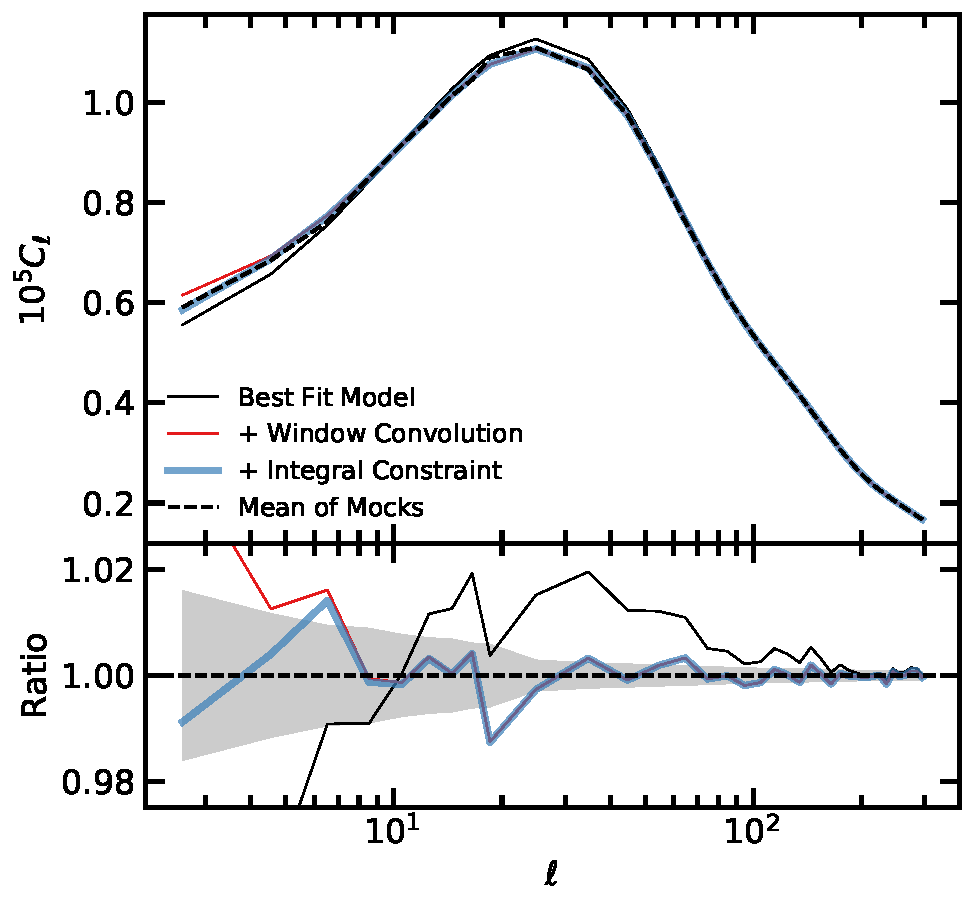
\includegraphics[width=0.5\textwidth]{model_mock.pdf}
\caption{Mean power spectrum of the lognormal density fields with $\fnl=0$ and best fit theoretical prediction after accounting for the survey geometry and integral constraint effects. Dark and light shades represent $1\sigma$ error on the mean and one realization, respectively. Bottom panel shows the residual power spectrum relative to the mean power spectrum of the mocks. No imaging systematic effects are added to these mocks.}\label{fig:model_mock}
\end{figure}

\subsubsection{Survey geometry and integral constraint}
The ensemble average for the partial sky power spectrum is related to that of the full sky power spectrum via the mode-mode coupling matrix $M_{\ell \ell^{\prime}}$ ,
\begin{equation}
    <\hat{C}_{\ell}> = \sum_{\ell^{\prime}} M_{\ell \ell^{\prime}}<C_{\ell^{\prime}}>.
\end{equation}
In general, the mode-mode coupling matrix is singular for a large sky cut, but a common approach is to use a discrete set of $\ell$ bins and assume the angular power spectrum is constant in each bin. This is not a bad assumption, but it might not be ideal for large scale modes and small bin widths. Therefore, we following a similar approach to \cite{chon2004fast}, and convolve the theoretical power spectrum $C_{\ell}$ with the survey mask window power to obtain the theoretical pseudo-power spectrum, rather than trying to de-convolve the observed power spectrum. The convolution in the spherical harmonics space becomes a multiplication in the correlation function space. To this end, we first estimate the paircount of the survey mask. The window paircount is normalized such that it is equal to one at the zero degree separation. Next, we multiply the model correlation function by the survey mask paircount. Then, the window-convolved power spectrum is obtained from,
\begin{align}
    \hat{C}^{\rm model}_{\ell} &= 2\pi \int \hat{\omega}^{\rm model}\hat{\omega}^{\rm mask}~P_{\ell}(\cos \theta) d\theta.
\end{align}

Finally, we account for the effect of integral constraint by subtracting the power spectrum of the survey mask,
\begin{equation}
     \hat{C}^{\rm model, IC}_{\ell} = \hat{C}^{\rm model}_{\ell} - \hat{C}^{\rm model}_{\ell=0} (\frac{\hat{C}^{\rm window}_{\ell}}{\hat{C}^{\rm window}_{\ell=0}}).
\end{equation}

We validate the pipeline for modeling the angular power spectrum against the lognormal simulations. Fig. \ref{fig:model_mock} shows the log-transformed mean of 1000 spectra from the simulations (dashed) and the best fit theory prediction before and after accounting for survey geometry and integral constraint. light and dark shades represent the 68\% error on the mean and one single realization, respectively. DESI footprint mask is applied to the mocks, and even though DESI covers around $40\%$ of the sky, but the window effect is affecting modes down to $\ell=200$. On the other hand, integral constraint only alters the power in the first two bins.

\subsection{Parameter estimation}
The signature of local PNG in the two-point function is unique and cannot be reproduced with other standard cosmological parameters. For parameter inference, we use standard Monte-Carlo Markov Chain sampling while allowing $\fnl$, shotnoise, and bias to vary. For the bias, we assume a constant clustering amplitude for our sample of LRGs, $b(z) = b/D(z)$, and fit for b. Throughout this manuscript, we use a discrete set of bandpower bins with $\Delta\ell=2$ between $\ell=2$ and $20$ and $\Delta \ell=10$ from $\ell=20$ to $300$, while weighting each mode by $2\ell+1$. We also find that the distribution of power spectrum at the lowest bin, $2\leq \ell < 12$,  is not Gaussian and its standard deviation varies significantly from mocks with $\fnl=0$ to those with $76.9$ (see, Fig. \ref{fig:histcell}). Therefore, we attempt to fit $\log C_{\ell}$ to make our constraints less sensitive to the choice of covariance matrix. The parameter $\fnl$ is constrained by maximizing a posterior defined as,
\begin{equation}
-2\ln\mathcal{L} = (\log C(\Theta)-\log \hat{C})^{\dagger} \mathbb{C}^{-1} (\log C(\Theta)-\log \hat{C}) + \chi^{2}_{\rm priors},
\end{equation}
where $\Theta$ represents the parameters, $\fnl$, bias coefficient, and shotnoise, all of which are associated with a flat prior, $\chi^{2}_{\rm priors}$; $C(\Theta)$ is the (binned) theoretical power spectrum including the effects for survey geometry and integral constraint; $\hat{C}$ is the (binned) measured power spectrum; and $\mathbb{C}$ is the covariance matrix constructed from simulations and corrected for the effect with Hartlap \mr{CITE}. 

\begin{figure}
\centering
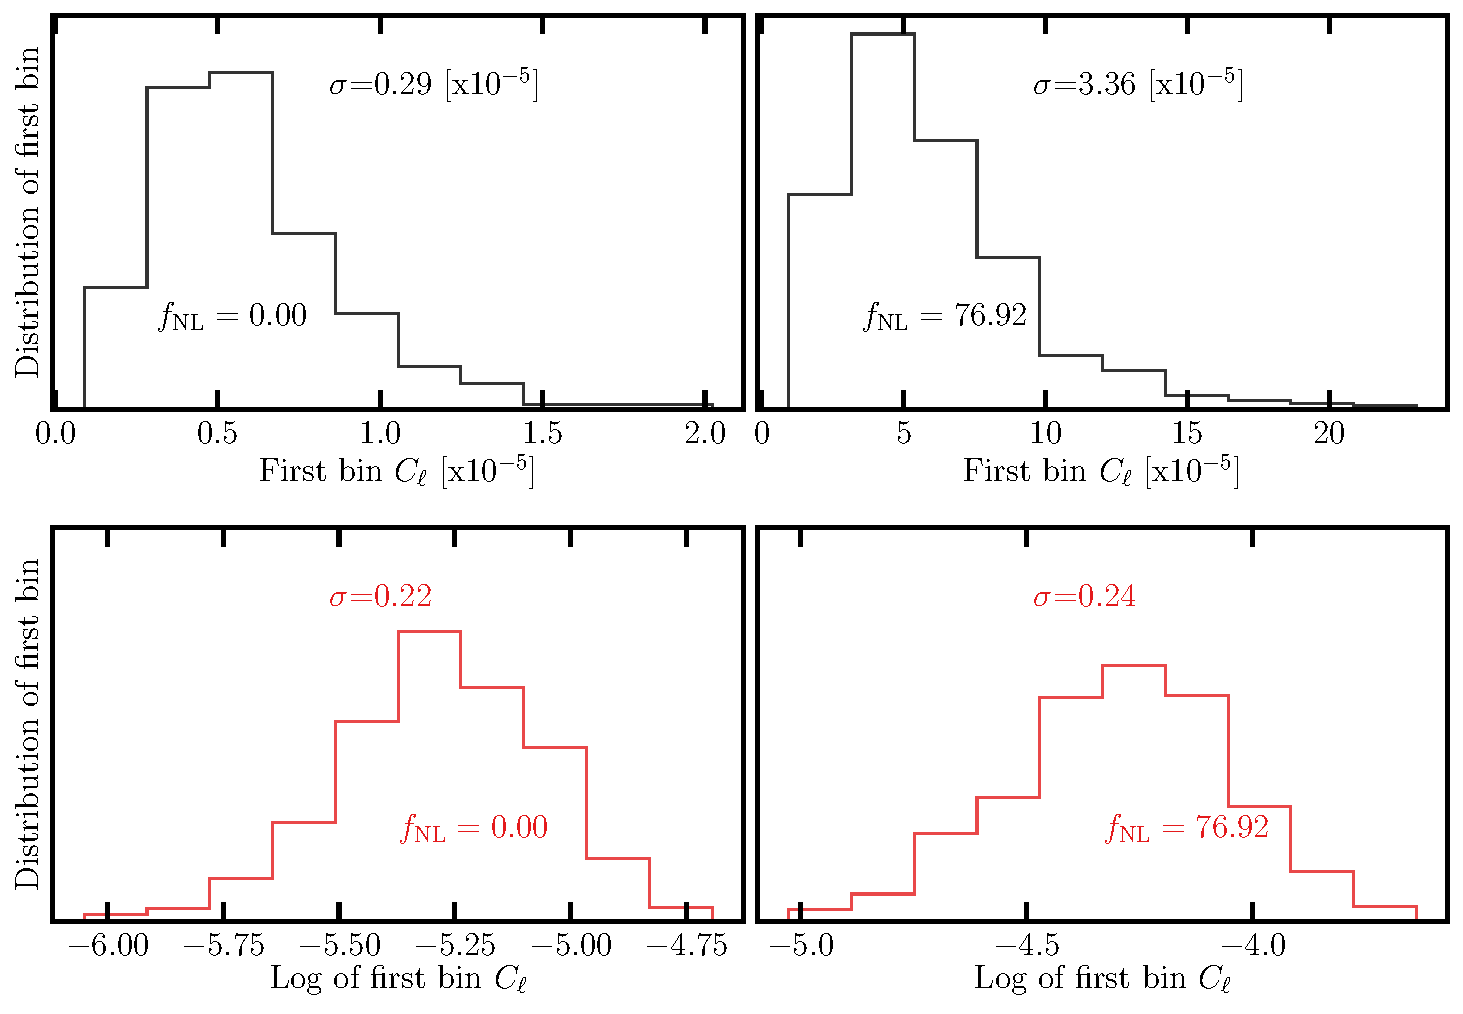
\includegraphics[width=0.5\textwidth]{hist_cl.pdf}
\caption{Distribution of the first bin power spectrum and its log transformation from the mocks with $\fnl=0$ (left) and $76.92$ (right). Differences in the standard deviations become less significant, and power spectrum measurements follow a more symmetric distribution after the log transformation.}\label{fig:histcell}
\end{figure}


\subsection{Remaining systematic errors}
\label{ssec:characterization}

In the absence of systematic effects, a) the mean density of galaxies should be uniform within the statistical fluctuations regardless of the imaging condition and b) the cross power spectrum between the galaxy density and imaging properties should be consistent with zero with statistical fluctuations. With these priors, we apply two statistical tests to look for remaining systematic effects in our sample of LRGs.

\begin{figure*}
\centering
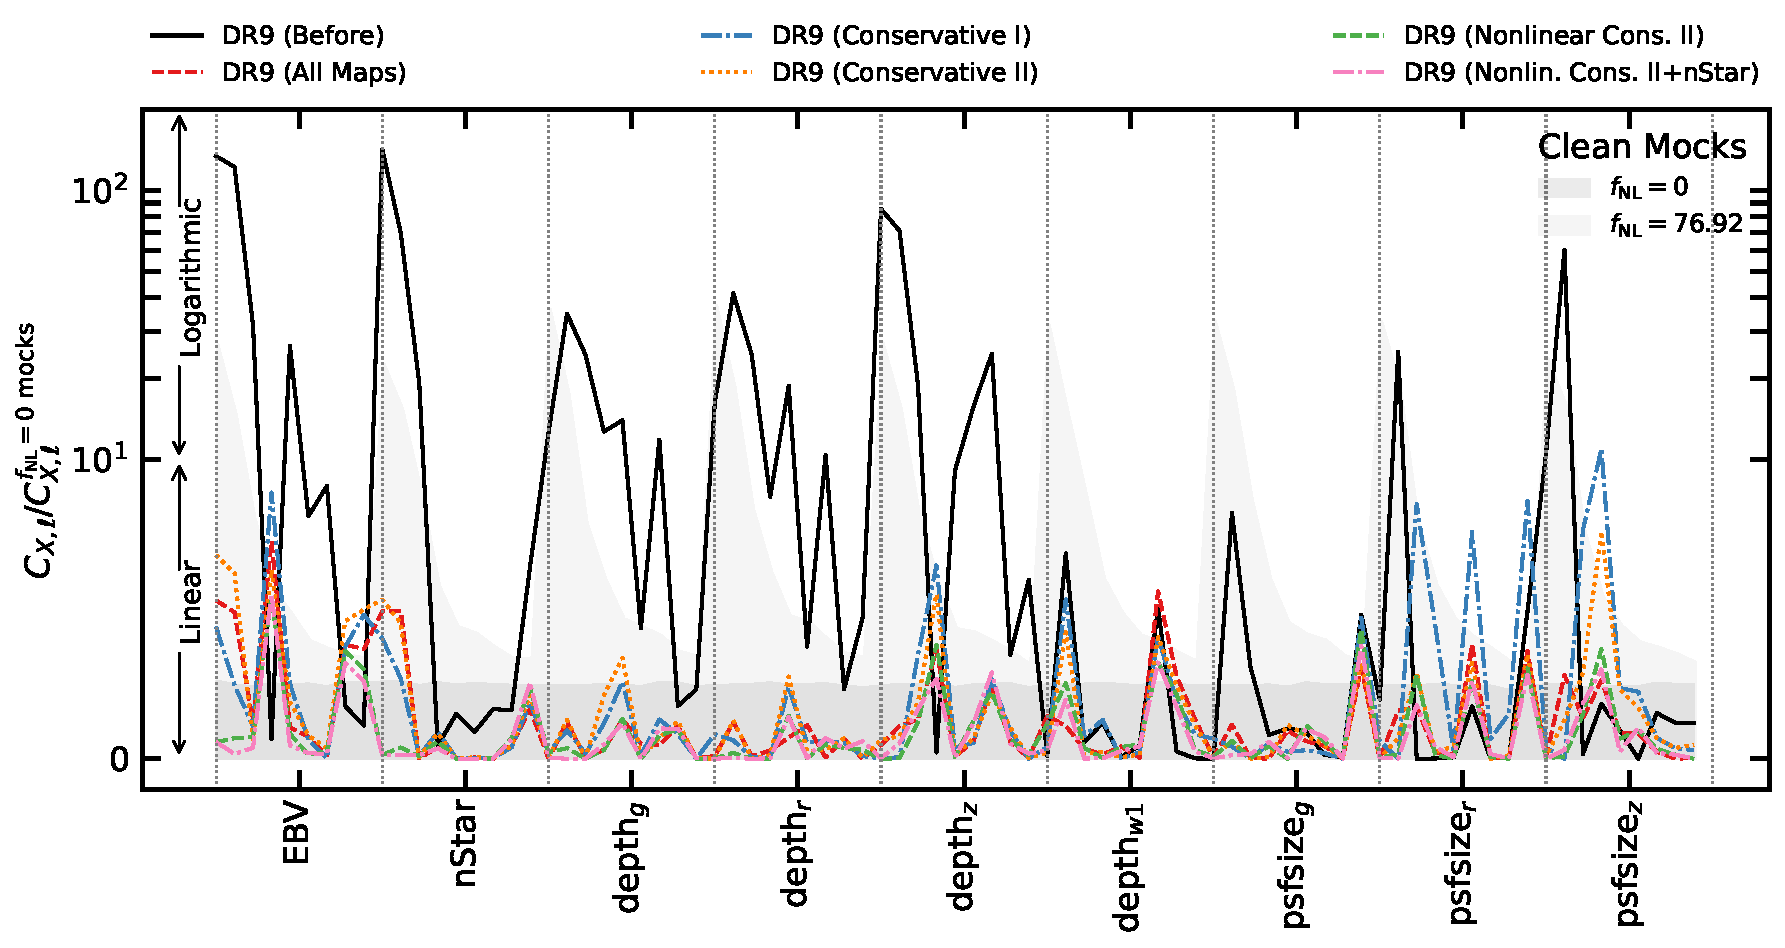
\includegraphics[width=0.76\textwidth]{clx_mocks.pdf}
\caption{Cross power spectra between the DR9 LRG sample and imaging maps. Dark and light shades represent the $97.5$ percentile of 1000 lognormal mocks without and with PNG, respectively.}\label{fig:clxmock}
\end{figure*}

\begin{figure*}
\centering
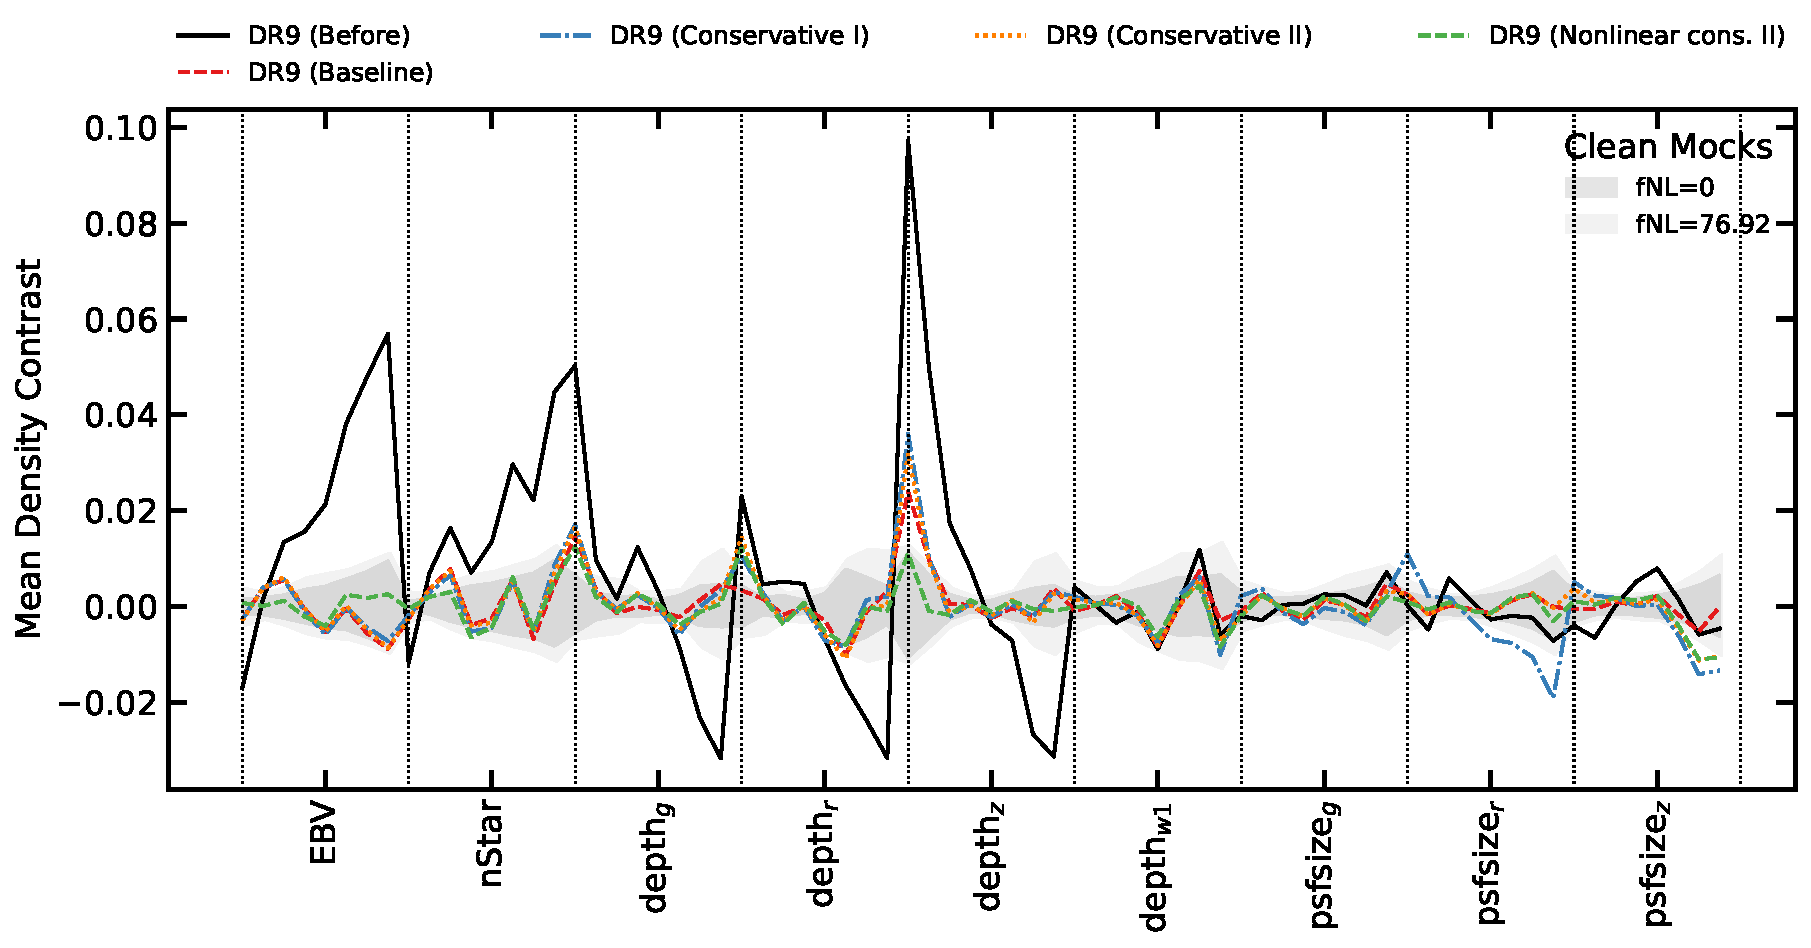
\includegraphics[width=0.76\textwidth]{nbar_mocks.pdf}
\caption{Mean density contrast of the DR9 LRG sample as a function of imaging maps. Dark and light shades represent the $1\sigma$ dispersion of 1000 lognormal mocks without and with PNG, respectively.}\label{fig:nbarmock}
\end{figure*}


\begin{figure}
\raggedleft
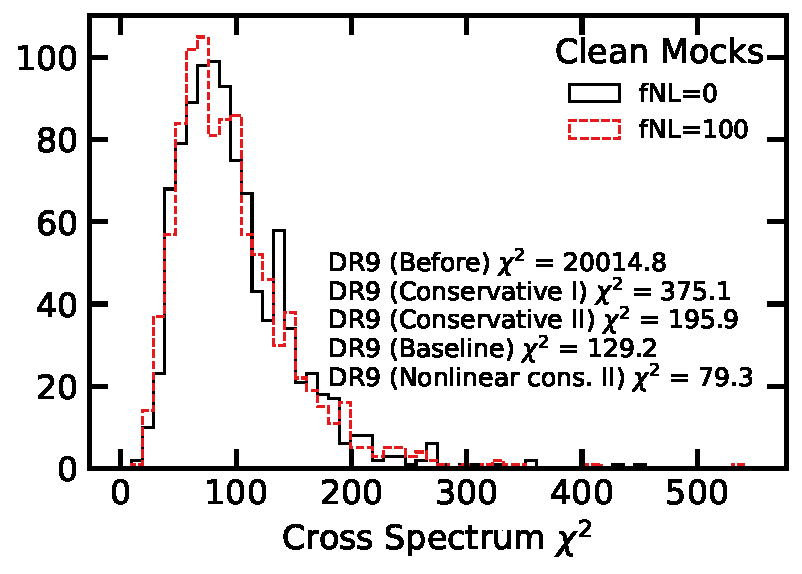
\includegraphics[width=0.45\textwidth]{chi2test.pdf}
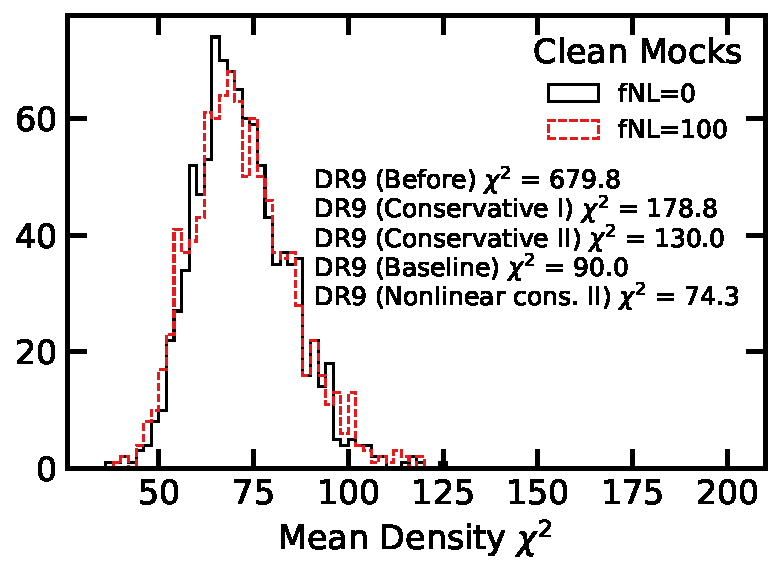
\includegraphics[width=0.44\textwidth]{chi2test2.pdf}
\caption{Remaining systematic error $\chi^{2}$ from the galaxy-imaging cross power spectrum (top) and the mean galaxy density contrast (bottom). The values observed in the DR9 sample before and after linear and nonlinear treatments are quoted, and the histograms are constructed from 1000 realizations of clean lognormal mocks with $\fnl=0$ and $76.92$.}\label{fig:chi2test}
\end{figure}


\subsubsection{Cross power spectrum}
We calculate the cross power spectra between galaxy density contrast field and imaging maps,
\begin{equation}
\hat{C}_{X, \ell} = [\hat{C}_{x_{1}, \ell}, \hat{C}_{x_{2}, \ell}, \hat{C}_{x_{3}, \ell}, ..., \hat{C}_{x_{9}, \ell}],
\end{equation}
where $C_{x_{i}, \ell}$ represents the cross power spectrum between the galaxy density and $i^{\rm th}$ imaging map, normalized by the auto power spectrum of $x_{i}$:
\begin{equation}
\hat{C}_{x_{i}, \ell} = \frac{(\hat{C}_{gx_{i}, \ell})^{2}}{\hat{C}_{x_{i}x_{i},\ell}}.
\end{equation}
Then, the $\chi^{2}$ value for the cross power spectra is calculated via,
\begin{equation}
\chi^{2} = \hat{C}^{T}_{X, \ell} \mathbb{C}_{X}^{-1} \hat{C}_{X, \ell},
\end{equation}
where the covariance matrix $\mathbb{C}_{X} = < \hat{C}_{X, \ell} \hat{C}_{X, \ell'} >$ is constructed from the lognormal mocks. This $\chi^{2}$ statistics is measured for every mock realization with the \textit{leave-one-out} technique\footnote{999 realizations are used to estimate the covariance matrix and applied to measure the $\chi^{2}$ for the left-out realization.}, and then is compared to the $\chi^{2}$ value observed from the DR9. We only use the bandpower bins from $\ell=2$ to $20$ with $\Delta\ell=2$, although higher modes are included for a robustness test later. 

Fig. \ref{fig:clxmock} shows the measured $C_{X}$ from the DR9 sample before and after applying various corrections for imaging systematics. The dark and light shades show the 97.5$^{\rm th}$ percentile from the $\fnl=0$ and $76.9$ mocks, respectively. The LRG sample has the highest cross correlation against the extinction, stellar density, and the z-band depth (solid black curve). As the most conservative cleaning approach, a linear model is trained with the extinction and z-band depth (\textit{linear conservative I}). With the correction applied, we find that the cross power spectrum against the r-band psftsize increases (dot-dashed blue curve), which indicates that only the extinction and the z-band depth are not sufficient to regress out all of the residual cross correlations between the LRG density and imaging. With the linear model re-trained using the three maps (\textit{linear conservative II}), we are able to reduce the cross power spectra (dotted orange curve). For comparison, we also show the cross spectra for a case in which the DR9 is cleaned using the linear model trained with all imaging maps (dashed red curve). There are minor differences between the \textit{linear conservative II} and \textit{linear all maps} cross spectra, further supporting the idea that only three imaging maps are sufficient to regress out spurious correlations.

Fig. \ref{fig:chi2test} (top) shows the histogram of the cross spectrum $\chi^{2}$ from 1000 mocks with and without $\fnl$. The $\chi^{2}$ values observed in the DR9 sample are quoted for comparison. Before cleaning, the DR9 sample has a cross power spectrum $\chi^{2}$ error of $20014.8$. After correction with the linear conservative I approach, the cross spectrum $\chi^{2}$ is reduced to $375.1$ with p-value $=0.002$. Adding the r-band psfsize, the linear model reduces the $\chi^{2}$ down to $195.9$ with p-value $=0.044$; we can reject the null hypothesis that the DR9 sample with the linear conservative II is properly cleaned at $95\%$ confidence. Although training the linear model with all imaging maps as input gives the lowest cross spectrum $\chi^{2}$ of $129.2$ (and p-value $=0.239$), but it potentially makes the analysis more prone to over-fitting and regressing out the true clustering signal, given the inner correlations among the imaging properties (see, Fig. \ref{fig:pcc}). As an alternative, we train the nonlinear method with the extinction, z-band depth, and r-band psfsize maps (\textit{nonlinear conservative II}) and clean the DR9 sample. The cross power spectrum $\chi^{2}$ is reduced to $79.3$ with p-value $=0.594$.  Adding the stellar density map reduces the cross power spectrum $\chi^{2}$ error to $70.9$ (p-value $=0.687$). This cross power spectrum diagnostic supports the idea that a nonlinear cleaning approach is desired to null out the remaining spurious fluctuations. We investigate cross spectrum to higher multipoles but find no evidence of remaining systematic error (see Appendix \ref{sec:scalesys}). 

\subsubsection{Mean density contrast}
We calculate the histogram of the mean density contrast relative to the $j^{\rm th}$ imaging property:
\begin{equation}
\delta_{x_{j}} = ({\hat{\overline{\rho}}})^{-1} \frac{\sum_{i} \rho_{i} f_{{\rm pix}, i}}{\sum_{i} f_{{\rm pix}, i}},
\end{equation}
where the summations are over \textsc{HEALPix} pixels in the bin with similar imaging values. For instance, In the absence of systematic error, the mean density contrast from one part of the sky with high extinction should be consistent with that from another patch with low extinction. We compute the histograms against all other imaging properties (see Fig. \ref{fig:ng}), and construct the total mean density contract as,
\begin{equation}
\delta_{X} = [\delta_{x_{1}}, \delta_{x_{2}}, \delta_{x_{3}}, ..., \delta_{x_{9}}],
\end{equation}
and the total residual error as,
\begin{equation}
\chi^{2} = \delta_{X}^{T} \mathbb{C_{\delta}}^{-1} \delta_{X},
\end{equation}
where the covariance matrix $\mathbb{C}_{\delta} = < \delta_{X} \delta_{X}>$ is constructed from the lognormal mocks. Fig. \ref{fig:nbarmock} shows the mean density contrast against the imaging properties for the DR9 LRG sample. The dark and light shades represent the $1\sigma$ level fluctuations observed in 1000 lognormal density fields respectively with $\fnl=0$ and $76.92$. The DR9 sample before treatment (solid curve) exhibits a strong trend around $10\%$ against the z-band depth which is consistent with the cross power spectrum. Additionally, there are significant spurious trends against the extinction and stellar density at about $5-6\%$. The linear approach is able to mitigate most of the systematic fluctuations with only the extinction and z-band depth as input maps; however,  a new trend appears against the r-band psfsize with the linear conservative I approach (dot-dashed blue curve), which is indicative of the psfsize-related systematics in the LRG sample. This finding is in agreement with the cross power spectrum. We re-train the linear model with three maps identified as \textit{conservative II}, but we still observe around $2\%$ residual spurious fluctuations in the low end of the z-band depth, which implies nonlinear systematic effects exist. We find that the nonlinear model trained with the three identified maps (or four maps including the stellar density) is capable of reducing the fluctuations below $2\%$. We experiment with different binning schemes but find consistent results.


Fig. \ref{fig:chi2test} (bottom) shows the mean density $\chi^{2}$ observed in the mocks with or without $\fnl$. We find consistent results regardless of the underlying $\fnl$, which supports that our diagnostic is not sensitive to the fiducial cosmology. The values measured in the DR9 sample before and after applying imaging weights are quoted for comparison. The \textit{linear conservative I} weights reduce the $\chi^{2}$ value from $679.8$ (before correction) to $178.8$. The p-value $=0$ indicates severe remaining systematic effects. Adding the r-band psfsize does not reduce the p-value enough (e.g., greater than $0.05$) even though the cleaning method yields a lower $\chi^{2}=130$. Training the linear model with all imaging maps returns a more reasonable $\chi^{2}=90$ and p-value of $0.084$; however, regression with all imaging maps as input can lead to the removal of the true clustering signal. We try the \textit{nonlinear conservative II} approach. We obtain a $\chi^{2}$ value of $74.3$ with p-value $=0.392$. Retraining the nonlinear approach while adding the stellar map yields minor improvement: $\chi^{2}=73.2$ and p-value $=0.422$.  This indicates that the stellar density trend in the mean density of LRGs can be explained via the extinction map.


\subsection{Calibration of mitigation bias}
The template-based mitigation of imaging systematics removes some of the true clustering signal, and the amount of the removed signal increases as more maps are fed to the regression. Below we describe an approach to calibrate our cleaning methods and de-bias our $\fnl$ constraints. 

\begin{figure}
\centering
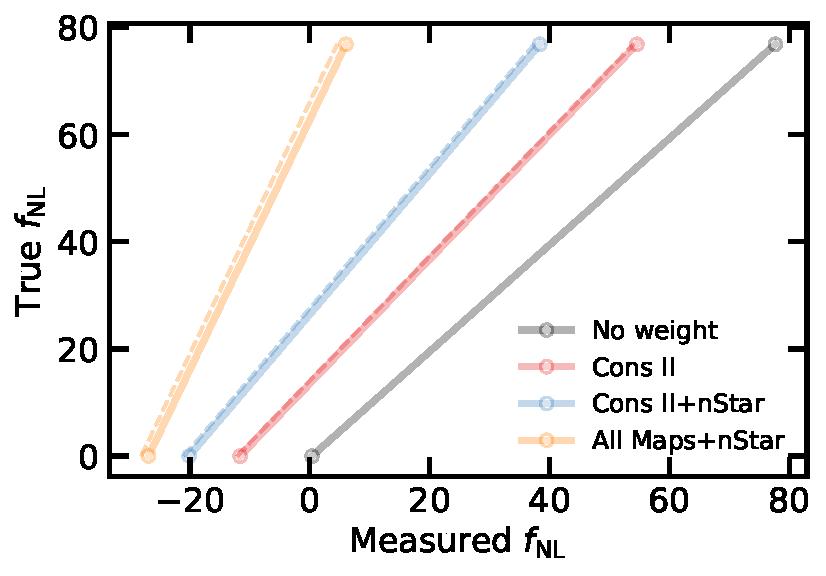
\includegraphics[width=0.45\textwidth]{figures/fnlbias}
\caption{True vs measured $\fnl$ values from the $\fnl=0$ and $76.9$ mocks with (dashed lines) and without systematics (solid lines). The lines represent the best fit estimates from fitting the mean power spectrum and the scatters show the best fit estimates from fitting individual spectra, only shown for the clean mocks for clarity.}\label{fig:fnlbias}
\end{figure}

We utilize our series of lognormal density fields with and without PNG, with and without systematic effects. The contamination models in the simulations are based on a linear multivariate model with the extinction, z-band depth, and r-band psfsize and are drawn from the sampled posterior constrained from fitting the DR9 sample. The idea is to simulate systematic effects that reflect realistic spurious fluctuations in the real data. For correction, the nonlinear model is trained and applied to the simulations with various sets of imaging maps as input, namely, we consider \textit{nonlinear conservative II}, \textit{nonlinear conservative II + nStar}, and \textit{nonlinear All Maps + nStar}. We fit the mean power spectrum and each individual power spectrum of 1000 realizations. The best fit estimates from the mocks without systematics (and no mitigation applied) are considered as the true $\fnl$ values and the estimates from the mocks with mitigation applied are considered as the measured values. Fig. \ref{fig:fnlbias} shows the true $\fnl$ values and the measured $\fnl$ values from fitting the mean power spectrum (solid lines) and individual spectra (points). The dashed lines show the best fit estimates from the contaminated realizations. The best fit estimates for the contaminated mocks before cleaning (\textit{no weight}) or per realizations are not shown for visual clarity. 

Then, a pair of linear coefficients are found to map the measured to the true values of $\fnl$, e.g., $f_{\rm NL, true} = m_{1} f_{\rm NL, measured} + m_{2}$. These coefficients for the mean power spectrum are summarized in Tab. \ref{tab:debiasparams}. The parameters for the \textit{All Maps+nStar} approach are the highest, as more mitigation bias is expected when more imaging maps are used. The value for $m_{1}-1$ determines the added uncertainty in the $\fnl$ inference due to mitigation, which is the highest for \textit{All Maps+nStar} and smallest for \textit{Conservative II}.

\begin{table}
\begin{center}
\caption{Linear parameters employed to de-bias the $\fnl$ constraints to account for the over-correction issue.}\label{tab:debiasparams}
\begin{tabular}{lcc}
\hline
\hline
\textbf{Cleaning Method} & $m_{1}$ & $m_{2}$ \\
\hline
Nonlinear Conservative II & 1.17 & 13.95 \\
Nonlinear Conservative II+nStar & 1.32 & 26.97 \\
Nonlinear All Maps+nStar & 2.35 & 63.5\\
\hline
\end{tabular}
\end{center}
\end{table}